\section{Ejercicio Resuelto}

A continuación resolvemos el problema de flujo resumido en la
Fig.~\ref{enu01}.  Se busca reproducir el flujo de agua en un suelo
isótropo que tiene un espesor de 9.2 metros, está formado por arena
limosa con coeficiente de permeabilidad ($k_x=k_y=k_z=5\cdot10^{-5}$
m/s) y limita en su parte inferior con una capa de arcilla
impermeable.  En este estrato arenoso se ha clavado 4.6 m de una
tablestaca que asumiremos de longitud infinita en la dirección
perpendicular al plano del dibujo. A la izquierda de la tablestaca
(aguasarriba) se ha acumulado una altura de 3 metros de agua y a la
derecha (aguas abajo) la escorrentía hace no haya acumulación de
agua. Para el problema así definido y asumiendo un régimen
estacionario se pide:
\begin{enumerate}
\item Obtener el caudal de agua saliente aguas abajo (por unidad de
  longitud de la dirección $y$).
\item Obtener la evolución de la carga total del fluido en el camino
  BCD y estimar el valor del gradiente hidráulico en el punto D.
\end{enumerate}

\begin{figure}[!h]
  \begin{center}
    \includegraphics[width=0.75\textwidth]{./body/images/enu01}
  \end{center}
  \caption{Descripción del modelo}
  \label{enu01}
\end{figure}

Las unidades que vamos a utilizar se resumen en el Cuadro \ref{tab:201}:
\begin{table}[!h]
  \centering
  \begin{tabular}{lc}
\hline
Magnitud&Unidades\\
\hline
  Longitud & m\\
  Altura total del fluido $h$ & m \\
  Coeficiente permeabilidad $k$ & m/s\\
  Vector flujo $\mathbf{q}$ & m$^3$/s/m$^2$ \\
  Gradiente hidráulico $\mathbf{i}_h$ & m/m \\
\hline
  \end{tabular}
  \caption{Unidades del problema}
  \label{tab:201}
\end{table}

Para resolver este problema iniciamos Abaqus como en la práctica del tema 1 y 
definimos un directorio de trabajo llamado \textit{Practica02}. A continuación
se describen las acciones a realizar en cada uno de los módulos para llevar
a cabo el análisis. 

\subsection{Módulo Part. Crear la geometría de los elementos}
Activamos el módulo \textit{Part} (ver Fig.~\ref{part01}) y creamos un
nuevo objeto tipo \textbf{2D Planar}, \textbf{Deformable} y
\textbf{Shell} (ver Fig.~\ref{part02}).

  \begin{figure}[!h]
    \centering
    \begin{subfigure}[!h]{0.29\textwidth}
      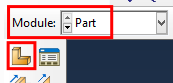
\includegraphics[width=\textwidth]{./body/images/part01.pdf}
      \caption{Inicio módulo \textbf{Part}}
      \label{part01}
    \end{subfigure}%
    ~ %add desired spacing between images, e. g. ~, \quad, \qquad, \hfill etc.
    % (or a blank line to force the subfigure onto a new line)
    \begin{subfigure}[!h]{0.39\textwidth}
      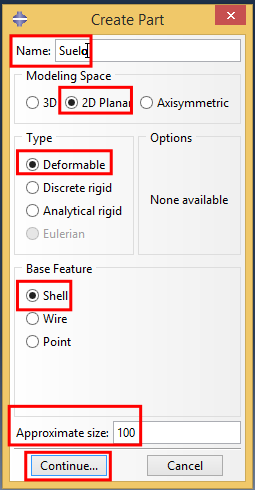
\includegraphics[width=\textwidth]{./body/images/part02.pdf}
      \caption{cuadro de diálogo \textbf{Create Part}}
      \label{part02}
    \end{subfigure}%
    \caption{Inicio módulo \textbf{Part} y cuadro de diálogo
      \textbf{Create Part}}
  \end{figure}
  Con la herramienta \textit{Sketcher} definimos la geometría del
  problema como indica la Fig.~\ref{part03} obteniendo finalmente la nueva
  \textit{part} que muestra la Fig.~\ref{part04}.
  \begin{figure}[!h]
    \centering
    \begin{subfigure}[!h]{1.0\textwidth}
      \includegraphics[width=\textwidth]{./body/images/part03}
      \caption{Definición de la geometría}
      \label{part03}
    \end{subfigure}%
    
  %add desired spacing between images, e. g. ~, \quad, \qquad, \hfill etc.
    % (or a blank line to force the subfigure onto a new line)
    \begin{subfigure}[!h]{0.875\textwidth}
      \includegraphics[width=\textwidth]{./body/images/part04}
      \caption{Nueva \textbf{Part}}
      \label{part04}
    \end{subfigure}%
    \caption{Construcción de una nueva \textbf{Part}}
  \end{figure}

  \subsection{Modulo Property. Definir materiales y secciones}

  Activamos ahora el módulo \textbf{Property} y definimos un nuevo
  material tipo \textbf{Thermal}, \textbf{Isotropic} y con una
  conductividad de $5\cdot 10^{-5}$ tal como muestras las
  Figs.\ref{prop01} a \ref{prop03}.
  \begin{figure}[!h]
    \centering
    \begin{subfigure}[!h]{0.22\textwidth}
      \includegraphics[width=\textwidth]{./body/images/prop01.pdf}
      \caption{Comando \textbf{Create Material}}
      \label{prop01}
    \end{subfigure}%
    ~ %add desired spacing between images, e. g. ~, \quad, \qquad, \hfill etc.
    % (or a blank line to force the subfigure onto a new line)
    \begin{subfigure}[!h]{0.36\textwidth}
      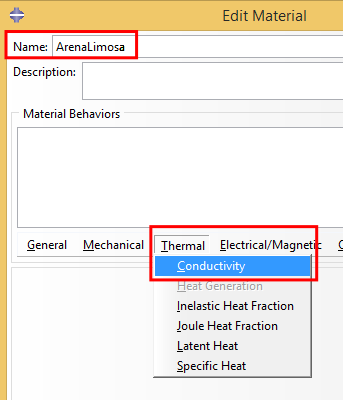
\includegraphics[width=\textwidth]{./body/images/prop02.pdf}
      \caption{Selección tipo de comportamiento}
      \label{prop02}
    \end{subfigure}%
    ~
    \begin{subfigure}[!h]{0.36\textwidth}
      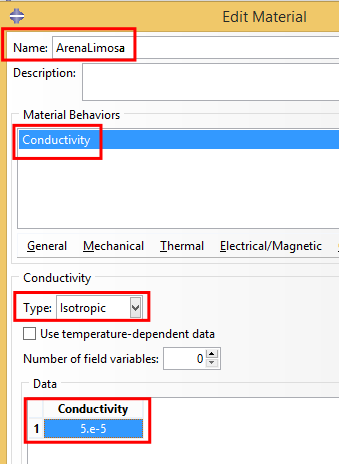
\includegraphics[width=\textwidth]{./body/images/prop03.pdf}
      \caption{Definición parámetros del material}
      \label{prop03}
    \end{subfigure}%
    \caption{Definición de un nuevo material}
  \end{figure}

  Una vez definido el material debemos definir una nueva sección de
  tipo \textbf{Solid} y \textbf{Homogeneous} siguiendo los pasos de
  las Figs.~\ref{prop03p} a \ref{prop05}.

  \begin{figure}[!h]
    \centering
    \begin{subfigure}[!h]{0.20\textwidth}
      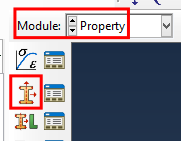
\includegraphics[width=\textwidth]{./body/images/prop03p.pdf}
      \caption{Comando \textbf{Create Section}}
      \label{prop03p}
    \end{subfigure}%
    ~
    \begin{subfigure}[!h]{0.39\textwidth}
      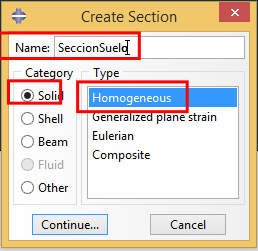
\includegraphics[width=\textwidth]{./body/images/prop04.pdf}
      \caption{Definición propiedades de la sección}
      \label{prop04}
    \end{subfigure}%
    ~ %add desired spacing between images, e. g. ~, \quad, \qquad, \hfill etc.
    % (or a blank line to force the subfigure onto a new line)
    \begin{subfigure}[!h]{0.39\textwidth}
      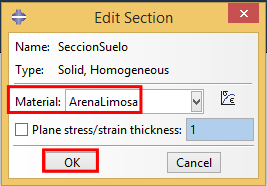
\includegraphics[width=\textwidth]{./body/images/prop05.pdf}
      \caption{Asignación del material a la sección}
      \label{prop05}
    \end{subfigure}%
    \caption{Definición de la sección \textit{SeccionSuelo}}
  \end{figure}

  Finalmente asignamos la sección creada a la \textbf{part} según se
  resume en las Figs.~\ref{prop05p} a \ref{prop07}.

  \begin{figure}[!h]
    \centering
    \begin{subfigure}[!h]{0.20\textwidth}
      \includegraphics[width=\textwidth]{./body/images/prop05p.pdf}
      \caption{Comando \textbf{Assign Section}}
      \label{prop05p}
    \end{subfigure}%
    ~
    \begin{subfigure}[!h]{0.39\textwidth}
      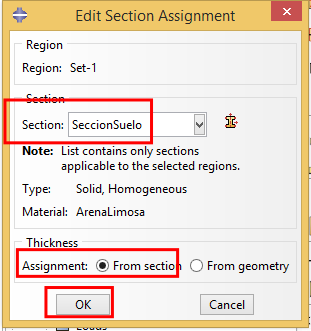
\includegraphics[width=\textwidth]{./body/images/prop06.pdf}
      \caption{Vinculación sección a \textit{Part}}
      \label{prop06}
    \end{subfigure}%
    
    % add desired spacing between images, e. g. ~, \quad, \qquad,
    % \hfill etc.
    % (or a blank line to force the subfigure onto a new line)
    \begin{subfigure}[!h]{0.75\textwidth}
      \includegraphics[width=\textwidth]{./body/images/prop07.png}
      \caption{\textit{Part} con sección asignada}
      \label{prop07}
    \end{subfigure}%
    \caption{Asignación de la sección a una \textbf{Part}}
  \end{figure}

  \subsection{Módulo Assembly. Ensamblar el modelo}

  En el módulo \textit{Assembly} ensamblamos nuestro modelo haciendo
  una copia \textbf{dependiente} de nuestra \textit{part} tal como
  indican las Figs.~\ref{asse01} y \ref{asse02}.

  \begin{figure}[!h]
    \centering
    \begin{subfigure}[!h]{0.25\textwidth}
      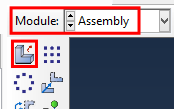
\includegraphics[width=\textwidth]{./body/images/asse01.pdf}
      \caption{Comando \textbf{Create Instance}}
      \label{asse01}
    \end{subfigure}%
    ~ %add desired spacing between images, e. g. ~, \quad, \qquad, \hfill etc.
    % (or a blank line to force the subfigure onto a new line)
    \begin{subfigure}[!h]{0.39\textwidth}
      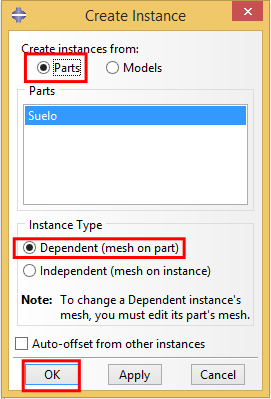
\includegraphics[width=\textwidth]{./body/images/asse02.pdf}
      \caption{Creación de una copia \textbf{Dependiente}}
      \label{asse02}
    \end{subfigure}%
    \caption{Acción \textbf{Create Instance}}
  \end{figure}

  \subsection{Módulo Step. Configurar el procedimiento de análisis}

  Necesitamos crear un caso de cálculo de tipo \textbf{Heat Transfer}
  indicando que va a ser \textbf{estacionario} (\textbf{Steady-state})
  (ver Figs.~\ref{step01} a \ref{step03}).


  \begin{figure}[!h]
    \centering
    \begin{subfigure}[!h]{0.20\textwidth}
      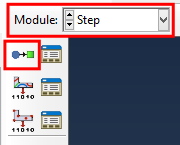
\includegraphics[width=\textwidth]{./body/images/step01.pdf}
      \caption{Comando \textbf{Create Step}}
      \label{step01}
    \end{subfigure}%
    ~
    \begin{subfigure}[!h]{0.39\textwidth}
      \includegraphics[width=\textwidth]{./body/images/step02.pdf}
      \caption{Propiedades nuevo caso de cálculo}
      \label{step02}
    \end{subfigure}%
    ~ %add desired spacing between images, e. g. ~, \quad, \qquad, \hfill etc.
    % (or a blank line to force the subfigure onto a new line)
    \begin{subfigure}[!h]{0.39\textwidth}
      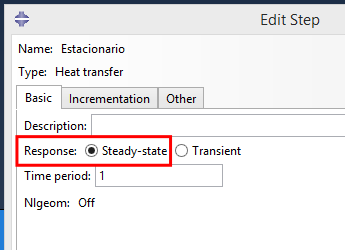
\includegraphics[width=\textwidth]{./body/images/step03.pdf}
      \caption{Selección análisis estacionario}
      \label{step03}
    \end{subfigure}%
    \caption{Creación de un nuevo caso de cálculo}
  \end{figure}

  Al haber haber definido un régimen estacionario Abaqus no nos
  genera un \textbf{History Output}. Revisemos entonces los datos que
  le vamos a pedir que nos guarde para el postproceso abriendo el
  \textbf{Field Output} que crea por defecto, y asegurándonos que
  guardamos las \textbf{temperaturas nodales}, el \textbf{vector de
    flujo de calor} y los \textbf{flujos de reacción} (allí donde
  aplicamos una condición de contorno tipo Dirchlet de temperatura)
  tal como indican las Figs.~\ref{step04} y \ref{step05}.

  \begin{figure}[!h]
    \centering
    \begin{subfigure}[!h]{0.45\textwidth}
      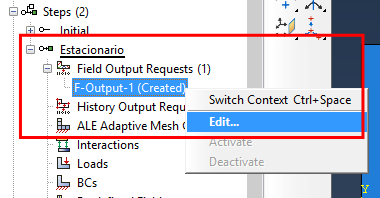
\includegraphics[width=\textwidth]{./body/images/step04.pdf}
      \caption{Selección del \textbf{Field Output}}
      \label{step04}
    \end{subfigure}%
    ~ %add desired spacing between images, e. g. ~, \quad, \qquad, \hfill etc.
    % (or a blank line to force the subfigure onto a new line)
    \begin{subfigure}[!h]{0.45\textwidth}
      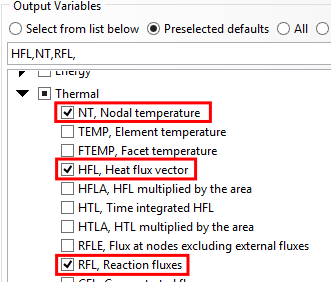
\includegraphics[width=\textwidth]{./body/images/step05.pdf}
      \caption{Valores a guardar para el postproceso}
      \label{step05}
    \end{subfigure}%
    \caption{Definición del \textit{Field Output}}
  \end{figure}

  \subsection{Módulo Load. Aplicar las condiciones de contorno}

  En el caso de problemas de flujo confinados podemos encontrar las
  siguientes dos condiciones de contorno (en nuestro problema
  impondremos un valor constante a las condiciones de contorno porque
  asumimos estamos en un régimen estacionario) :
  \begin{description}
  \item[Tipo esencial] Contornos donde imponemos el valor de la carga
    total del fluido $h=h^*$.
  \item[Tipo natural] Contorno donde imponemos el valor del flujo
    $(-\textbf{k}\cdot\bm{\nabla}h)\cdot\textbf{n}=\mathrm{cte}$,
    siendo $\textbf{n}$ la normal exterior al contorno donde imponemos
    el valor del flujo.
  \end{description}

  Si no imponemos nada en un contorno de nuestro dominio, Abaqus
  entiende que estamos imponiendo que el flujo a través de esa
  frontera es nulo (frontera impermeable), lo que se traduce que
  estamos imponiendo $ \bm{\nabla}h\cdot\textbf{n}=0$.

  En nuestro caso tenemos que imponer:
  \begin{enumerate}
  \item Dos condiciones de contorno tipo esencial en la parte
    superior del dominio (asumiendo que el datum está en la línea
    horizontal AE)
    \begin{itemize}
    \item $h=u_A/\gamma_w+z_A=\dfrac{\rho_w\; g\; 3}{\rho_w g}+0 = 3$
      m en la equipotencial AB
    \item $h=u_E/\gamma_w+z_E= \dfrac{\rho_w\; g\; 0}{\rho_w g}+0=0$ m
      en la equipotencial DE
    \end{itemize}
    Estas condiciones las impondremos en el caso de carga creado he
    hemos llamado \textit{estacionario}.
  \item La condición de contorno tipo natural de frontera impermeable $
    \bm{\nabla}h\cdot\textbf{n}=0$ en los contornos AGFE y BCD. Esta
    condición de contorno se mantiene fija en todo el análisis y la
    podríamos definir en el caso de carga creado por Abaqus
    \textit{Initial} para que se propague al resto de casos de
    carga. Sin embargo, como esta condición (frontera impermeable) se
    define por defecto, no es necesario que definamos nada.
  \end{enumerate}

  Para imponer la condición de contorno tipo esencial $h=3$ en el
  contorno AB activamos el módulo \textbf{Load} y pulsamos la orden
  \textbf{Create Boundary Condition} (ver Fig.~\ref{load02}). Después
  sigue las instrucciones indicadas en las Figs.~\ref{load03} a
  \ref{load05}.

  \begin{figure}[!h]
    \centering
    \begin{subfigure}[!h]{0.25\textwidth}
      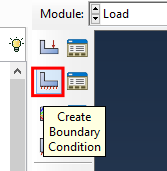
\includegraphics[width=\textwidth]{./body/images/load02.pdf}
      \caption{Comando \textbf{Create Boundary Condition}}
      \label{load02}
    \end{subfigure}%
    ~ %add desired spacing between images, e. g. ~, \quad, \qquad, \hfill etc.
    % (or a blank line to force the subfigure onto a new line)
    \begin{subfigure}[!h]{0.45\textwidth}
      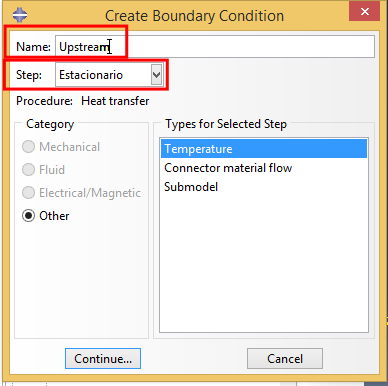
\includegraphics[width=\textwidth]{./body/images/load03.pdf}
      \caption{Definición tipo de condición esencial}
      \label{load03}
    \end{subfigure}%

    \begin{subfigure}[!h]{0.52\textwidth}
      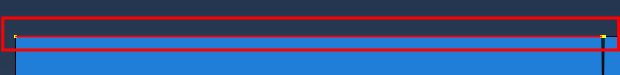
\includegraphics[width=\textwidth]{./body/images/load04.pdf}
      \caption{Selección de la frontera}
      \label{load04}
    \end{subfigure}%
    ~ %add desired spacing between images, e. g. ~, \quad, \qquad, \hfill etc.
    % (or a blank line to force the subfigure onto a new line)
    \begin{subfigure}[!h]{0.45\textwidth}
      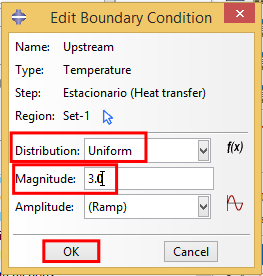
\includegraphics[width=\textwidth]{./body/images/load05.pdf}
      \caption{Definición de la altura total impuesta}
      \label{load05}
    \end{subfigure}%
    \caption{Definición de la condición de contorno en la
      equipotencial AB}
  \end{figure}

  De igual manera, para imponer las condición de contorno tipo
  esencial $h=0$ en el contorno DE sigue las instrucciones indicadas
  en las Figs.~\ref{load06} a \ref{load08}. Al final Abaqus indica las
  fronteras donde has impuesto las condiciones de contorno tal como
  muestra la Fig.~\ref{load09}.

  \begin{figure}[!h]
    \centering
    \begin{subfigure}[!h]{0.42\textwidth}
      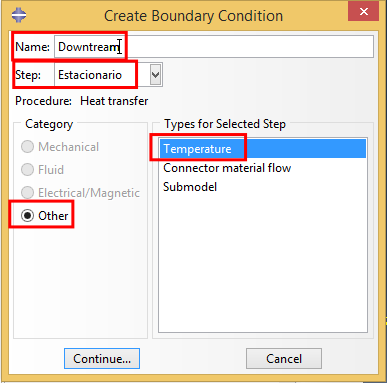
\includegraphics[width=\textwidth]{./body/images/load06.pdf}
      \caption{Definición tipo de condición esencial}
      \label{load06}
    \end{subfigure}%
    ~ %add desired spacing between images, e. g. ~, \quad, \qquad, \hfill etc.
    % (or a blank line to force the subfigure onto a new line)
    \begin{subfigure}[!h]{0.55\textwidth}
      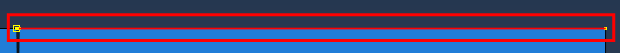
\includegraphics[width=\textwidth]{./body/images/load07.pdf}
      \caption{Selección de la frontera}
      \label{load07}
    \end{subfigure}%

    \begin{subfigure}[!h]{0.42\textwidth}
      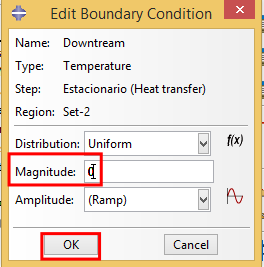
\includegraphics[width=\textwidth]{./body/images/load08.pdf}
      \caption{Definición de la altura total impuesta}
      \label{load08}
    \end{subfigure}%
    ~ %add desired spacing between images, e. g. ~, \quad, \qquad, \hfill etc.
    % (or a blank line to force the subfigure onto a new line)
    \begin{subfigure}[!h]{0.55\textwidth}
      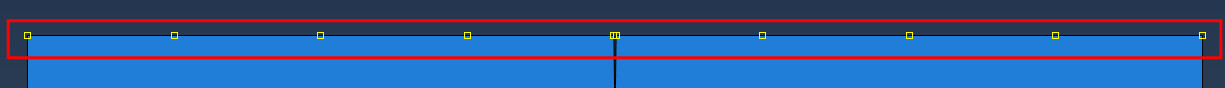
\includegraphics[width=\textwidth]{./body/images/load09.pdf}
      \caption{Indicación fronteras con condiciones impuestas}
      \label{load09}
    \end{subfigure}%
    \caption{Definición de la condición de contorno en la
      equipotencial DE}
  \end{figure}


  \subsection{Módulo Mesh. Crear la malla.}

  Para construir la malla recordamos los pasos a seguir tal como se
  indicaron en la práctica 1:
  \begin{enumerate}
  \item Activo el módulo \textbf{Mesh} y, dado que hemos ensamblado el
    modelo con una copia dependiente, impongo que voy a mallar la
    \textbf{part} tal como indica la Fig.\ref{mess01}.
    \begin{figure}[!h]
      \begin{center}
        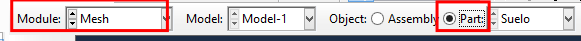
\includegraphics[width=0.9\textwidth]{./body/images/mess01.pdf}
      \end{center}
      \caption{Inicio del módulo \textbf{mesh}}
      \label{mess01}
    \end{figure}
  \item Defino la forma del elemento (serán cuadriláteros) (ver
    Fig.~\ref{mess02}).
    \begin{figure}[!h]
      \begin{center}
        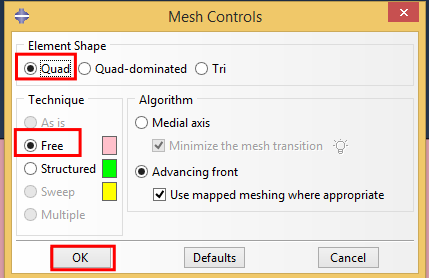
\includegraphics[width=0.45\textwidth]{./body/images/mess02.pdf}
      \end{center}
      \caption{Definición forma del elemento}
      \label{mess02}
    \end{figure}
  \item Defino el tamaño global del elemento a 1.5 metros (ver
    Fig.~\ref{mess03})
    \begin{figure}[!h]
      \begin{center}
        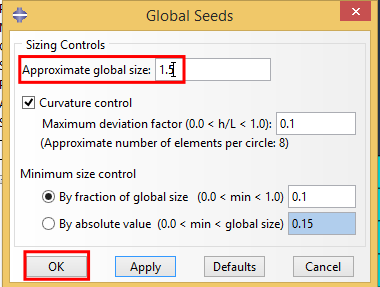
\includegraphics[width=0.45\textwidth]{./body/images/mess03.pdf}
      \end{center}
      \caption{Definición tamaño del elemento}
      \label{mess03}
    \end{figure}
  \item Finalmente defino el tipo de interpolación tal como indica la
    Fig.\ref{mess04}.
    \begin{figure}[!h]
      \begin{center}
        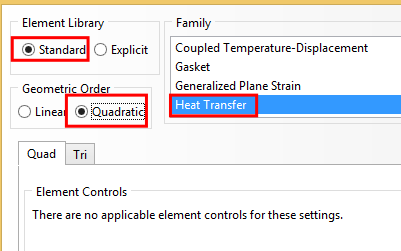
\includegraphics[width=0.45\textwidth]{./body/images/mess04.pdf}
      \end{center}
      \caption{Definición interpolación del elemento}
      \label{mess04}
    \end{figure}
  \end{enumerate}

  La malla final se muestra en la Fig.~\ref{mess05}.
  \begin{figure}[!h]
    \begin{center}
      \includegraphics[width=0.85\textwidth]{./body/images/mess05}
    \end{center}
    \caption{Malla final}
    \label{mess05}
  \end{figure}

  \subsection{Módulo Job. Crear el trabajo y lanzar el análisis.}

  Tras definir el modelo sólo nos falta crear y lanzar el trabajo
  (\textbf{job}). Para hacerlo activa el módulo \textbf{job}, pulsa el
  icono \textbf{Create job} (ver Fig.~\ref{job01}) y sigue las
  instrucciones de las Figs.~\ref{job02} y \ref{job03}.
  \begin{figure}[!h]
    \centering
    \begin{subfigure}[!h]{0.21\textwidth}
      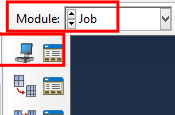
\includegraphics[width=\textwidth]{./body/images/job01.pdf}
      \caption{Comando \textbf{Create Job}}
      \label{job01}
    \end{subfigure}%
    ~ %add desired spacing between images, e. g. ~, \quad, \qquad, \hfill etc.
    % (or a blank line to force the subfigure onto a new line)
    \begin{subfigure}[!h]{0.32\textwidth}
      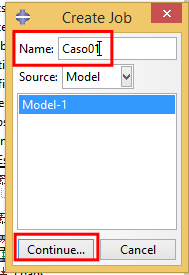
\includegraphics[width=\textwidth]{./body/images/job02.pdf}
      \caption{Cuadro de diálogo \textit{Create Job}}
      \label{job02}
    \end{subfigure}%
    ~
    \begin{subfigure}[!h]{0.44\textwidth}
      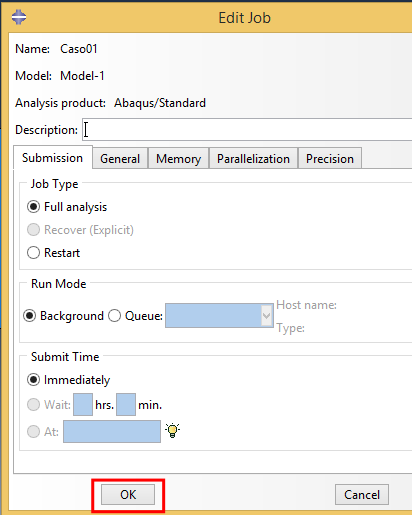
\includegraphics[width=\textwidth]{./body/images/job03.pdf}
      \caption{Parámetros del análisis}
      \label{job03}
    \end{subfigure}%
    \caption{Definición caso de cálculo}
  \end{figure}

  Finalmente lanza el trabajo y, una vez convergido el análisis
  numérico, activa el postproceso (ver Figs.~\ref{job04} y
  \ref{job05}).

  \begin{figure}[!h]
    \centering
    \begin{subfigure}[!h]{0.42\textwidth}
      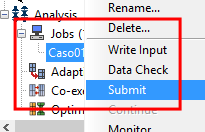
\includegraphics[width=\textwidth]{./body/images/job04.pdf}
      \caption{Lanzamiento del caso de cálculo}
      \label{job04}
    \end{subfigure}%
    ~ %add desired spacing between images, e. g. ~, \quad, \qquad, \hfill etc.
    % (or a blank line to force the subfigure onto a new line)
    \begin{subfigure}[!h]{0.42\textwidth}
      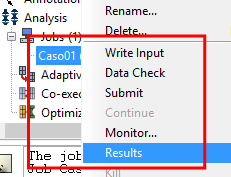
\includegraphics[width=\textwidth]{./body/images/job05.pdf}
      \caption{Activación postproceso}
      \label{job05}
    \end{subfigure}%
    \caption{Ejecución del caso de cálculo}
  \end{figure}

  \subsection{Módulo Visualization. Realizar el post-proceso.}
  A continuación se resumen las acciones a realizar en el postproceso
  para responder a las preguntas del enunciado:
  \begin{itemize}
  \item Dibujemos inicialmente el campo de la altura total del fluido
    en cada punto (ver Figs.~\ref{post01} y \ref{post02}). Si
    quisiéramos obtener las líneas de equipotenciales, activamos el
    comando \textbf{Contour Plot Options} y seleccionamos que el tipo
    de \textit{contour} sea \textbf{line} como indican las
    Figs.~\ref{post03} y \ref{post04}.

  \begin{figure}[!h]
    \centering
    \begin{subfigure}[!h]{0.21\textwidth}
      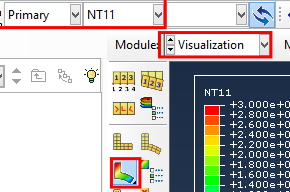
\includegraphics[width=\textwidth]{./body/images/post01.pdf}
      \caption{Comando \textbf{Plot Contours on deformed shape}}
      \label{post01}
    \end{subfigure}%
    ~ %add desired spacing between images, e. g. ~, \quad, \qquad, \hfill etc.
    % (or a blank line to force the subfigure onto a new line)
    \begin{subfigure}[!h]{0.60\textwidth}
      \includegraphics[width=\textwidth]{./body/images/post02}
      \caption{Distribución de la altura total del fluido}
      \label{post02}
    \end{subfigure}%

    \begin{subfigure}[!h]{0.40\textwidth}
      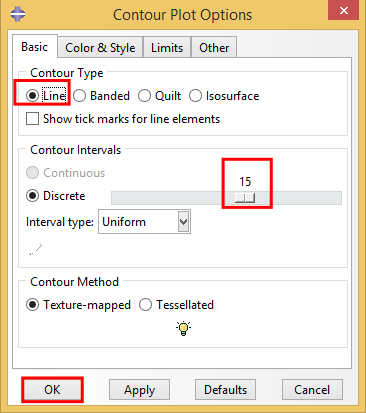
\includegraphics[width=\textwidth]{./body/images/post03.pdf}
      \caption{Cuadro de diálogo de \textbf{Contour Plots}}
      \label{post03}
    \end{subfigure}%
    \begin{subfigure}[!h]{0.60\textwidth}
      \includegraphics[width=\textwidth]{./body/images/post04}
      \caption{Distribución de la altura total del fluido}
      \label{post04}
    \end{subfigure}%
    \caption{Visualización de la altura total del fluido}
  \end{figure}

\item Buscamos responder ahora la primera de las preguntas del
  ejercicio, obtener el flujo saliente aguas abajo. Para hacerlo
  debemos obtener la distribución del flujo saliente en la recta DE e
  integrarlo. Definamos primero un \textbf{path} en el contorno DE que
  llamaremos \textit{CorrienteAbajo} tal como muestran las
  Figs.~\ref{post03} a \ref{post05}.

  \begin{figure}[!h]
    \centering
    \begin{subfigure}[!h]{0.20\textwidth}
      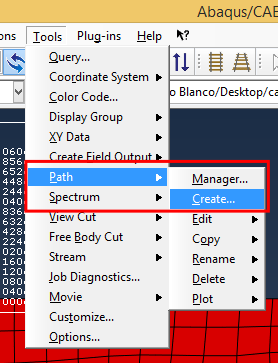
\includegraphics[width=\textwidth]{./body/images/post05.pdf}
      \caption{Comando \textbf{Path/Create}}
      \label{post05}
    \end{subfigure}%
    \begin{subfigure}[!h]{0.40\textwidth}
      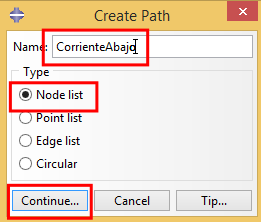
\includegraphics[width=\textwidth]{./body/images/post07.pdf}
      \caption{Cuadro de diálogo \textit{Create Path}}
      \label{post07}
    \end{subfigure}%
    \begin{subfigure}[!h]{0.40\textwidth}
      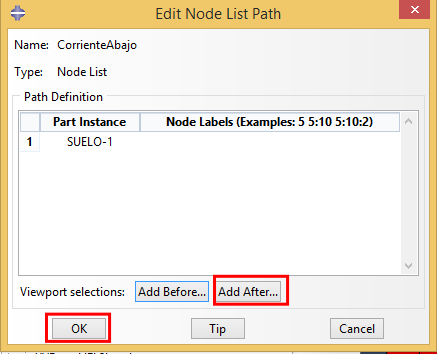
\includegraphics[width=\textwidth]{./body/images/post08.pdf}
      \caption{Definición geometría del \textit{path}}
      \label{post08}
    \end{subfigure}%
    
    \begin{subfigure}[!h]{0.60\textwidth}
      \includegraphics[width=\textwidth]{./body/images/post09}
      \caption{Frontera de aguas abajo}
      \label{post09}
    \end{subfigure}%
    \begin{subfigure}[!h]{0.40\textwidth}
      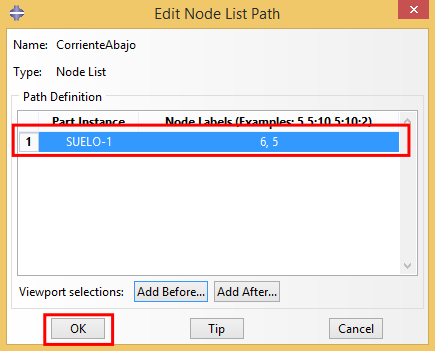
\includegraphics[width=\textwidth]{./body/images/post10.pdf}
      \caption{Definición geometría del \textit{path}}
      \label{post10}
    \end{subfigure}%
    \caption{Definición path \textit{AguasAbajo}}
  \end{figure}

\item Una vez definido el \textit{path}, buscamos obtener la
  distribución de la altura total sobre él. Para hacerlo debemos crear
  un objeto \textbf{XY Data} tal como resumen las Figs.\ref{post11} a
  \ref{post15}.
  \begin{figure}[!h]
    \centering
    \begin{subfigure}[!h]{0.21\textwidth}
      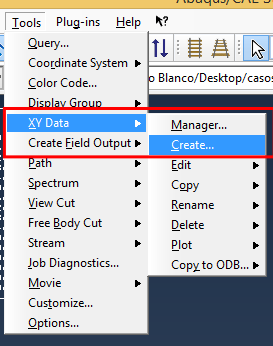
\includegraphics[width=\textwidth]{./body/images/post11.pdf}
      \caption{Comando \textbf{XY Data/Create}}
      \label{post11}
    \end{subfigure}%
    \begin{subfigure}[!h]{0.35\textwidth}
      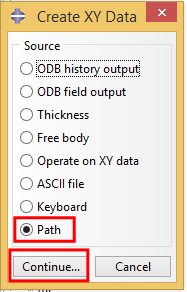
\includegraphics[width=\textwidth]{./body/images/post12.pdf}
      \caption{Cuadro de diálogo \textit{XY Data}}
      \label{post12}
    \end{subfigure}%
    \begin{subfigure}[!h]{0.44\textwidth}
      \includegraphics[width=\textwidth]{./body/images/post13.pdf}
      \caption{Cuadro de diálogo \textit{XY Data from path}}
      \label{post13}
    \end{subfigure}%
    
    \begin{subfigure}[!h]{0.60\textwidth}
      \includegraphics[width=\textwidth]{./body/images/post14.pdf}
      \caption{Selección de la variable a dibujar en el path}
      \label{post14}
    \end{subfigure}%
    \begin{subfigure}[!h]{0.40\textwidth}
      \includegraphics[width=\textwidth]{./body/images/post15.pdf}
      \caption{Cuadro de diálogo \textit{XY Data from path}}
      \label{post15}
    \end{subfigure}%
    \caption{Definición objeto XY Data con la altura total sobre el
      contorno DE}
  \end{figure}

\item La distribución del flujo saliente en el contorno DE se muestra
  en la Fig.~\ref{post16}. Para poder exportarlo luego a una hoja
  excel (e integrarlo) debemos guardarlo tal como muestran las
  Figs.~\ref{post17} y \ref{post18}.

  \begin{figure}[!h]
    \centering
    \begin{subfigure}[!h]{0.80\textwidth}
      \includegraphics[width=\textwidth]{./body/images/post16}
      \caption{Distribución flujo saliente en recta DE}
      \label{post16}
    \end{subfigure}%
    
    \begin{subfigure}[!h]{0.30\textwidth}
      \includegraphics[width=\textwidth]{./body/images/post17.pdf}
      \caption{Cuadro de diálogo \textit{Save XY Data As}}
      \label{post17}
    \end{subfigure}\quad
    \begin{subfigure}[!h]{0.30\textwidth}
      \includegraphics[width=\textwidth]{./body/images/post18.pdf}
      \caption{Objetos XY Data en el \textit{Model Tree}}
      \label{post18}
    \end{subfigure}%
    \caption{Objeto XY Data del flujo saliente en recta DE}
  \end{figure}

\item A continuación exportamos los datos del objeto XY Data que
  acabamos de crear tal como indican las Figs.~\ref{post19} a
  \ref{post21}.
  \begin{figure}[!h]
    \centering
    \begin{subfigure}[!h]{0.25\textwidth}
      \includegraphics[width=\textwidth]{./body/images/post19.pdf}
      \caption{Comando \textbf{Report/XY}}
      \label{post19}
    \end{subfigure}%
    \begin{subfigure}[!h]{0.37\textwidth}
      \includegraphics[width=\textwidth]{./body/images/post20.pdf}
      \caption{Cuadro de diálogo \textit{report XY Data}}
      \label{post20}
    \end{subfigure}%
    \begin{subfigure}[!h]{0.37\textwidth}
      \includegraphics[width=\textwidth]{./body/images/post21.pdf}
      \caption{Cuadro de diálogo \textit{report XY Data}}
      \label{post21}
    \end{subfigure}%
    \caption{Guardar en fichero tipo texto los datos del objeto XY
      Data}
  \end{figure}

\item A continuación se resume cómo importar el fichero de texto que
  acabamos de guardar en Excel. La información que contiene las
  Figs.~\ref{post22} a \ref{post25} es válida para Excel2013.
  \begin{figure}[!h]
    \centering
    \begin{subfigure}[!h]{0.50\textwidth}
      \includegraphics[width=\textwidth]{./body/images/post22.pdf}
      \caption{Importar datos de fichero texto en excel I}
      \label{post22}
    \end{subfigure}%
    \begin{subfigure}[!h]{0.50\textwidth}
      \includegraphics[width=\textwidth]{./body/images/post23.pdf}
      \caption{Importar datos de fichero texto en excel II}
      \label{post23}
    \end{subfigure}%

    \begin{subfigure}[!h]{0.50\textwidth}
      \includegraphics[width=\textwidth]{./body/images/post24.pdf}
      \caption{Importar datos de fichero texto en excel III}
      \label{post24}
    \end{subfigure}%
    \begin{subfigure}[!h]{0.50\textwidth}
      \includegraphics[width=\textwidth]{./body/images/post25.pdf}
      \caption{Importar datos de fichero texto en excel IV}
      \label{post25}
    \end{subfigure}%
    \caption{Importar datos de fichero texto en excel}
  \end{figure}

\item Con los datos importados, integramos la curva flujo \textit{vs.}
  distancia usando el método del trapecio obteniendo, finalmente, un
  valor del caudal saliente de $7.67\cdot 10^{-5}$ m$^3$/s por metro en
  la dirección $y$ (ver Fig.~\ref{post26}).
  \begin{figure}[!h]
    \begin{center}
      \includegraphics[width=0.99\textwidth]{./body/images/post26}
    \end{center}
    \caption{Integración del flujo total por el método del trapecio}
    \label{post26}
  \end{figure}

  De forma equivalente (y más rápida) podríamos haber integrado la
  curva de la Fig.~\ref{post16} usando la consola de \texttt{python}
  que tiene Abaqus. El objeto XY-Data que hemos llamado XYData-HFL2
  (ver Fig.~\ref{post18}) es un objeto que Abaqus guarda y que podemos
  acceder a él y con el que podemos operar, tal como muestra la
  Fig.~\ref{post26b} (intenta como ejercicio entender la lógica del
  código python mostrado).
  \begin{figure}[!h]
    \begin{center}
      \includegraphics[width=0.99\textwidth]{./body/images/post26b.pdf}
    \end{center}
    \caption{Integración del flujo total por el método del trapecio
      usando \texttt{python}}
    \label{post26b}
  \end{figure}

  Finalmente, hay una tercera forma de integrar esta curva usando los propios comandos de Abaqus, que nos permite operar con objetos \textit{XYData} previamente creados. Pulsamos \textit{Tools/XYData/Create}, pero en vez de crear un objeto nuevo según un \textit{path} eligiremos la opción \textit{Operate on XYData}, tal como muestra la Fig.~\ref{post26c}
   \begin{figure}[!h]
    \begin{center}
      \includegraphics[width=0.99\textwidth]{./body/images/post26c.pdf}
    \end{center}
    \caption{Selección de la herramienta \textit{Operate on XYData}}
    \label{post26c}
  \end{figure}

  De todas las operaciones posibles seleccionamos el comando \textit{integrate(X)} tomando como argumento el objeto \textit{XYData} donde hemos guardado el flujo normal a la superficie como resume la Fig.~\ref{post26d}
    \begin{figure}[!h]
    \begin{center}
      \includegraphics[width=0.99\textwidth]{./body/images/post26d.pdf}
    \end{center}
    \caption{Integración del objeto \textit{XYData}}
    \label{post26d}
  \end{figure}

Por último podemos dibujar el valor del flujo y su integración a lo largo de la curva tal como muestra la Fig.~\ref{post26e} y acceder al valor del flujo total para la ordenada final como muestra la Fig.~\ref{post26f}.
     \begin{figure}[!h]
    \begin{center}
      \includegraphics[width=0.99\textwidth]{./body/images/post26e.pdf}
    \end{center}
    \caption{Variación del flujo y su integración a lo largo del \textit{path}}
    \label{post26e}
  \end{figure}
      \begin{figure}[!h]
    \begin{center}
      \includegraphics[width=0.99\textwidth]{./body/images/post26f.pdf}
    \end{center}
    \caption{Integración del flujo a lo largo del \textit{path}}
    \label{post26f}
  \end{figure}
  
\item La segunda pregunta del enunciado nos pide obtener la evolución
  de la carga total del fluido en el camino BCD y estimar el valor del
  gradiente hidráulico en el punto D. Para ello debemos obtener la
  distribución de la carga hidráulica total en el camino BCD y estimar
  su pendiente en el punto D. De forma similar al punto anterior,
  definamos primero un \textbf{path} siguiendo el camino BCD tal como
  se resume en las Figs.~\ref{post27} a \ref{post30}.
  \begin{figure}[!h]
    \centering
    \begin{subfigure}[!h]{0.50\textwidth}
      \includegraphics[width=\textwidth]{./body/images/post27.pdf}
      \caption{Cuadro de diálogo \textit{Create Path}}
      \label{post27}
    \end{subfigure}%
    \begin{subfigure}[!h]{0.50\textwidth}
      \includegraphics[width=\textwidth]{./body/images/post28.pdf}
      \caption{Definición geometría del \textit{Path}}
      \label{post28}
    \end{subfigure}%

    \begin{subfigure}[!h]{0.07\textwidth}
      \includegraphics[width=\textwidth]{./body/images/post29}
      \caption{Frontera BCD}
      \label{post29}
    \end{subfigure}\quad%
    \begin{subfigure}[!h]{0.60\textwidth}
      \includegraphics[width=\textwidth]{./body/images/post30.pdf}
      \caption{Definición geometría del \textit{Path}}
      \label{post30}
    \end{subfigure}%
    \caption{Definición path \textit{CaminoBCD}}
  \end{figure}

\item Una vez definido el path \textit{CaminoBCD} debemos crear el
  objeto XY Data con la distribución de la carga hidráulica total
  según el camino BCD tal como resumen las Figs.~\ref{post31} a
  \ref{post34}.  La Fig.~\ref{post34} es la distribución pedida.
  \begin{figure}[!h]
    \centering
    \begin{subfigure}[!h]{0.33\textwidth}
      \includegraphics[width=\textwidth]{./body/images/post31.pdf}
      \caption{Cuadro de diálogo \textit{XY Data from path}}
      \label{post31}
    \end{subfigure}%
    \begin{subfigure}[!h]{0.33\textwidth}
      \includegraphics[width=\textwidth]{./body/images/post32.pdf}
      \caption{Selección de la variable a dibujar en el path}
      \label{post32}
    \end{subfigure}%
    \begin{subfigure}[!h]{0.33\textwidth}
      \includegraphics[width=\textwidth]{./body/images/post33.pdf}
      \caption{Cuadro de diálogo \textit{XY Data from path}}
      \label{post33}
    \end{subfigure}%

    \begin{subfigure}[!h]{0.80\textwidth}
      \includegraphics[width=\textwidth]{./body/images/post34}
      \caption{Distribución carga total hidráulica en BCD}
      \label{post34}
    \end{subfigure}%
    \caption{Objeto XY Data de la carga total en el camino BCD}
  \end{figure}

\item Podríamos estimar el gradiente hidráulico en la
  Fig.~\ref{post34} pero si quisiéramos calcularlo de forma exacta
  debemos guardar los datos en un objeto XY Data y luego exportarlos a
  un fichero texto tal como se resume en las Figs.\ref{post35} a
  \ref{post37}. De la Fig.\ref{post37} podemos calcular el gradiente
  pedido como:
  \begin{equation}
    \label{eq:02}
    i_h=\frac{0.3234-0}{9.2-7.67}=0.211
  \end{equation}

   \begin{figure}[!h]
     \centering
     \begin{subfigure}[!h]{0.33\textwidth}
       \includegraphics[width=\textwidth]{./body/images/post35.pdf}
       \caption{Guardar Objeto XY-Data}
       \label{post35}
     \end{subfigure}%
     \begin{subfigure}[!h]{0.33\textwidth}
       \includegraphics[width=\textwidth]{./body/images/post36.pdf}
       \caption{Exportar a fichero de texto objeto XY Data}
       \label{post36}
     \end{subfigure}%
     \begin{subfigure}[!h]{0.33\textwidth}
%       \includegraphics[width=\textwidth]{./body/images/post37.pdf}
       \includegraphics[width=\textwidth]{./body/images/29c.jpg}
       \caption{Valores fichero de texto}
       \label{post37}
     \end{subfigure}%
     \caption{Guardar objeto XY Data como fichero de texto}
   \end{figure}

   En este caso hubiese sido más sencillo pedir la información sobre
   el objeto XY Data creado (en el \textbf{Model Tree}, ver
   Figs.\ref{post38} y \ref{post39}) en vez de guardarlo en disco como
   un fichero texto.
   \begin{figure}[!h]
     \centering
     \begin{subfigure}[!h]{0.45\textwidth}
       \includegraphics[width=\textwidth]{./body/images/post38}
       \caption{Acceso directo a un objeto XY data en el \textbf{Model
           Tree}}
       \label{post38}
     \end{subfigure}\quad%
     \begin{subfigure}[!h]{0.450\textwidth}
%       \includegraphics[width=\textwidth]{./body/images/post39}
       \includegraphics[width=\textwidth]{./body/images/30b.jpg}
       \caption{Datos del objeto \textit{XYData-h}}
       \label{post39}
     \end{subfigure}%
     \caption{Información guardada en objeto \textit{XY Data}}
   \end{figure}
 \end{itemize}

 \hspace{20mm}\hrulefill$\star$\hrulefill\hspace{20mm}
